\documentclass[11pt]{amsart}

\usepackage{amsfonts, amsthm, amssymb, amsmath}
\usepackage{comment}
\usepackage{tikz-cd}
\usepackage{graphicx}
\usepackage{xurl}
\usepackage{xcolor}

\usetikzlibrary{snakes}

\usepackage{unicode-math}
\usepackage{fontspec}
\setmathfont{latinmodern-math.otf}
\setmathfont[range=\varnothing]{Asana-Math.otf}

\setlength{\textwidth}{6.5in}
\setlength{\oddsidemargin}{-0.1in}
\setlength{\evensidemargin}{-0.1in}

\input{commands}

\numberwithin{equation}{section}
\newtheorem{theorem}{Theorem}
\numberwithin{theorem}{section}
\newtheorem{theoremx}[theorem]{Theorem}
\newtheorem{lemma}[theorem]{Lemma}
\newtheorem{lemmax}[theorem]{Lemma}
\newtheorem{corollary}[theorem]{Corollary}
\newtheorem{proposition}[theorem]{Proposition}
\newtheorem{conjecture}[theorem]{Conjecture}
\newtheorem{problem}[theorem]{Problem}
\newtheorem{assumption}[theorem]{Assumption}
\newtheorem{defprop}[theorem]{Definition/Proposition}

\theoremstyle{definition}
\newtheorem{remark}[theorem]{Remark}
\newtheorem{exercise}[theorem]{Exercise}
\newtheorem{warning}[theorem]{Warning}
\newtheorem{definition}[theorem]{Definition}
\newtheorem{question}[theorem]{Question}
\newtheorem{example}[theorem]{Example}
\newtheorem{examples}[theorem]{Examples}
\newtheorem{observation}[theorem]{Observation}

\date{\today}

\setcounter{tocdepth}{1}

\title{Sofa Designers}

\author{Jineon Baek}

\begin{document}

\maketitle

\section{Introduction}
The \emph{moving sofa problem} was first proposed by Leo Moser in 1966 \cite{moser1966problem}.
Quoting directly from \cite{kallus2018improved, romik2018differential}, the problem asks the following:
\begin{problem}[Moving Sofa Problem]
What is the planar shape of maximal area that can be moved around a right-angled corner in a hallway of unit width?
\end{problem} 
Any planar shape that can be moved around such a hallway is called a \emph{sofa}.

The problem gained a noticeable attention from the mathematics community since \cite{romik2018differential} since its introduction, and major progresses have been made over time. However, the full problem remains unsolved to this date after 50 years.

In 1997, Gerver \cite{gerver1992moving} constructed a sofa of area $2.2195\dots$ and conjectured that it attains the maximum possible area.
The sofa's boundary consists of 3 line segments and 15 analytic curves, making its derivation complicated.

The goal of this project is to prove that the Gerver's sofa indeed attains the maximum possible area of a sofa.
As the work is still in progress, we restrict our attention to sofas that rotate 90 degrees at this moment. 
Our plan is to extend the argument to sofas that rotate in arbitrary angle 
\begin{remark}
For the rest of the document, we only focus on sofas that rotate by full 90 degrees.
\end{remark}

The introduction of each chapter is written so that, when only the introductions are read sequentially, will outline the overall strategy of the proof.
The subsections are meant to fill the mathematical provide details, which can be omitted for the first read.

\subsection{History}

% add figure with caption here
% known as Hammersley's sofa, can be moved around with a continuous mix of rotation and transition.

\subsubsection{Sofa Construction}
The area of an explicit sofa gives a lower bound of the maximum sofa area. 
Since the problem was introduced, sofas of area $2.2074\dots $ (by Hammersley \cite{hammersley1968enfeeblement}), $2.21563\dots$ (by C. Francis \cite{guy1977monthly}) and $2.215649\dots$ (by R. Guy \cite{guy1977monthly}) were successively constructed over time. 
In 1997, Gerver \cite{gerver1992moving} found the sofa of currently best known area $2.2195\dots$ by considerations of the local maximality of a sofa.
The boundary of Gerver's sofa consists of 3 line segments and 15 analytic curves, making its derivation complicated.
Romik \cite{romik2018differential} simplified the derivation of Gerver's sofa in his work on ambidextrous sofa.

\begin{comment}
\begin{figure}[hbt]
  \includegraphics[width=0.9\textwidth]{img/gerver.png}
  \caption{Gerver's sofa with 3 line segments (V, XVIII, XIII) and 15 analytic curves. Shamefully copied from Wikipedia (need to put credit).}
  \label{fig:gerver}
\end{figure}
\end{comment}

\subsubsection{Upper Bound of Sofa Area}
On the other hand, the current best known upper bound $2.37$ of sofa area is found by Kallus and Romik in 2017 \cite{kallus2018improved} by a computer-assisted proof.
It is conjectured that the Gerver's sofa indeed attains the maximum sofa area, a speculation held by authors worked on this problem \cite{gerver1992moving, romik2018differential} that is supported experimentally by gradient descent computation on the problem's polygonal variant \cite{gibbs2014computational}.
Thus, under the assumption that Gerver's sofa, the resolution of moving sofa problem boils down to improving the upper bound of possible sofa area.

\input{notations}

\section{Monotone Sofas}

In this section, we build up the notion of \emph{monotone sofas}, a subset of all sofas with additional structure on its shape and movement.

In terms of geometry, a monotone sofa $S$ consists of its \emph{cap} $\cC(S)$, a convex set of a particular shape, subtracted by the sofa's \emph{niche} $\cD(S)$, a uncountable union of triangles.
In terms of movement, a monotone sofa always rotates clockwise while touching the outer sides $a$ and $c$ of the hallway $L$.

\textcolor{red}{Add figure here}

We will prove that any sofa of maximum area is always a monotone sofa minus a measure zero set.
Therefore, it suffices to bring our attention to monotone sofas only. 

Monotone sofas have specific geometric properties that makes it easy to analyze. 
Also, the set of monotone sofas can be embedded as a convex subset of an affine space easily.
A monotone sofa $S$ is determined by the path of the hallway's inner corner $\xx \colon [0, \pi / 2] \ra \RR^2$ in sofa view.
It turns out that the condition for path $\xx$ to generate a monotone sofa is convex, so that .
Therefore, we can generate 

\subsection{Monotone Sofas}
\textcolor{red}{Under construction. The following text comes from previous writings and needs to undergo major changes.}

Take any sofa $S$. The starting observation is that for the canonical movement of $S$, the intersection (\ref{eq:intersection}) is connected and thus already a sofa that encloses $S$.

\begin{theorem}
\label{thm:normal-sofa}
For the canonical movement of a sofa $S$, the intersection $N(S)$ defined as Equation (\ref{eq:intersection}) is connected, and so is a sofa that contains $S$. 
\end{theorem}
Call this sofa $N(S)$ as the \emph{normalization} of $S$, and any sofa of such form a \emph{normal sofa}. 
By the restricted motion of canonical movement, a normal sofa will have much richer properties than an arbitrary sofa. We first introduce relevant notations for further discussions.

\begin{definition}
For each $t \in [0, \beta]$, let $a(t)$, $b(t)$, $c(t)$ and $d(t)$ be the sides of $L_t$ corresponding to the sides $a, b, c$ and $d$ of $L$ (so that for example, $a(t) = f^{-1}_t(a)$).


\end{definition}

Now we move back to the proof of connectedness of $N(S)$.
\begin{proof} (of Theorem \ref{thm:normal-sofa})
Fix an arbitrary point $p \in N(S)$.
We will show that there is a line segment inside $N(S)$ connecting $p$ to a point in $S$. This completes the proof of connectedness of $N(S)$, as $N(S)$ is the union of $S$ with line segments extending from $S$.

Let $l_\theta$ be the line parallel to the $x$-axis rotated counterclockwise by an arbitrary angle $\theta \in [\beta, \pi / 2]$. 
Regardless of $\theta$, the intersection $s_\theta = l_\theta \cap N(S)$ is either a line segment or an empty set. This is because $s_\theta$ is the intersection of $l_\theta \cap H$, $l_\theta \cap (\Rot_\beta(V) + \xx(\beta))$, and $l_\theta \cap L_t$ for all $t \in [0, \beta]$, each a line segment contained in $l_\theta$.

Now it only remains to show that for some $\theta$, $l_\theta$ overlaps with $S$ so that $s_\theta$ connects $p$ with a point in $S$. 
If either one of $l_\beta$ or $l_{\pi / 2}$ overlaps with $S$, we are done. 
Assume otherwise that none of $l_\beta$ and $l_{\pi / 2}$ overlaps with $S$.
Since $S$ is connected, it is either on the left side of $l_{\pi / 2}$ or the right side of $l_{\pi / 2}$.
As we are working with the canonical movement of $S$, $S$ touches the side $a(0)$ of $L_0$ inside $L_0$. This implies that $S$ is on the right side of $l_{\pi / 2}$.
A similar argument with the side $c(\beta)$ of $L_\beta$ shows that $S$ is on the left side of $l_\beta$.
Now move $l_\theta$ continuously, taking $\theta$ from $\beta$ to $\pi / 2$. As $S$ is on the different sides of $l_\theta$ for $\theta = \beta$ and $\pi / 2$, at some point $S$ will cross the boundary $l_\theta$ for some $\theta$. This completes the proof of connectedness.

The conditions that $N(S)$ are contained in $L_t$ and rotated strips of $L$ and $V$ follow naturally from the definition \ref{eq:intersection}.
Thus $N(S)$ is a valid sofa.
\end{proof}


It is worth noting that the normalization of a normal sofa is itself.
That is, the normalization is a projection from the collection of sofas to the collection of normal sofas.
\begin{corollary}
\label{cor:norm-proj}
Take any sofa $S$. 
The canonical movement of $S$ that \emph{defines} the normal sofa $N(S)$ as in (\ref{eq:intersection}) is identical to the canonical movement \emph{of} the normal sofa $N(S)$.
Consequently, for any normal sofa $S$, $N(S) = S$.
\end{corollary}
\begin{proof}
By definition, the canonical movement $f_t$ (the continuum of isometries that move a sofa) of $S$ is a valid movement of $N(S)$. 
Since $N(S) \supset S$, the moving copy $f_t(N(S))$ is rotated clockwise by $t$ and always touches the sides $a$ and $c$ of $L$.
This identifies $f_t$ with the canonical movement of $N(S)$.
\end{proof}

With this, it is natural for us to work with normal sofas only as normalizing a sofa does not decrease the area.

\subsection{General shape of a normal sofa}
\textcolor{red}{Under construction. The following text comes from previous writings and needs to undergo major changes.}
Normal sofas conform to a specific geometric configuration. 
We introduce definitions and theorems that describe the general shape of a normal sofa. See Figure xx for the accompanying figure.

\begin{definition}
For any $t \in \RR$, let $u_t = (\cos t, \sin t)$ and $v_t = (- \sin t, \cos t)$.
The basis $u_t, v_t$ of $\RR^2$ follows the frame of rotating hallway $L_t$. 
\end{definition}

\begin{definition}
Let $Q^+ = (-\infty, 1] \times (-\infty, 1]$ and $Q^- = (-\infty, 0) \times (-\infty, 0)$.
With this, $L = Q^+ \setminus Q^-$.

For an arbitrary, fixed normal sofa $S$ with angle of rotation $\beta$ and canonical movement $f_t$, let $Q^+_t = f^{-1}_t(Q^+)$ and $Q^-_t = f^{-1}_t(Q^-)$.
$Q_t^+$ is the closed plane quadrant under the lines $c(t)$ and $a(t)$.
$Q_t^-$ is the open plane quadrant under the lines $d(t)$ and $b(t)$.
$L_t$ is $Q_t^+ \setminus Q_t^-$.

Let $V_\beta$ be the rotated vertical strip $\Rot_\beta(V) + \xx(\beta)$.
Let $P = H \cap V_\beta$. This is equal to $H$ for $\beta = \pi / 2$ and 
is a parallelogram with two heights equal to 1 and an angle of $\beta + \pi / 2$ for $\beta < \pi / 2$.
Let $\cC$ be the convex set $P \cap \bigcap_{t=0}^\beta Q_t^+$.
Let $\cD$ be the set $P \cap \bigcup_{t=0}^\beta Q_t^-$.
With this, $S = \cC \setminus \cD$.
\end{definition}

Since we are working with the canonical movement of $S$, $a(t)$ and $c(t)$ for all $t \in [0, \beta]$ are tangent lines of $S$ from above. 
$a(t)$ forms an angle of $t$ from the $y$-axis, and $c(t)$ forms the angle of $t$ from the $x$-axis.
Consequently, $\cC$ is a bounded convex set with tangent lines $a(t)$ and $c(t)$ for all $0 \leq t \leq \beta$ from above and sides $b(\beta)$ and $d(0)$ from below.
Define $\partial \cC$ as the boundary segment of $\cC$ touched by lines $a(t)$ and $c(t)$ for all $0 \leq t \leq \beta$.
Then $\partial \cC$ is a continuous curve consisting of two convex segments, each with tangent lines $\{a(t)\}_{0 \leq t \leq \beta}$ and $\{c(t)\}_{0 \leq t \leq \beta}$ respectively, joined at the vertex $a(\beta) \cap c(0)$ of $P$ for $\beta < \pi / 2$ or the segment $\partial \cC \cap c(0)$ for $\beta = \pi / 2$. 
The endpoints of $\partial \cC$ are $E_{l} = c(\beta) \cap b(\beta)$ and $E_{r} = a(0) \cap d(0)$ .
This, with the theorem below, characterizes the shape of a normal sofa.
\begin{theorem}
\label{thm:normal-structure}
$\cD$ is a subset of $\cC \setminus \partial \cC$.
\end{theorem}
\begin{proof} (sketch)
Let $\cF$ be the fan above the line $b(\beta)$ and $d(0)$ with vertex $O = b(\beta) \cap d(0)$.
We only need to show that $P \cap Q^-_t$ is contained in $\cC \setminus \partial \cC$ for all $0 < t < \beta$.
When $\xx(t)$, the corner of $Q_t^-$, is not in $\cF$, $P \cap Q^-_t$ is empty and we are done.

So assume $\xx(t) \in \cF$. There are three possible configurations of $Q_t^-$ in $\cF$. \textcolor{blue}{Figure here}.
In all three cases, we only need to show the followings for all :
\begin{enumerate}
	\item The point $F_l = d(t) \cap b(\beta)$ is on the strictly right side of the endpoint $E_l$ of $\partial \cC$ in $b(\beta)$.
	\item The point $F_r = b(t) \cap d(0)$ is on the strictly left side of the endpoint $E_r$ of $\partial \cC$ in $c(0)$.
	\item The point $\xx(t)$ is inside $\cC$.
\end{enumerate}
We first show that (1) holds.
Say that a point $p_0$ is further than $p_1$ in the direction of nonzero vector $v \in \RR^2$ if and only if $p_0 \cdot v > p_1 \cdot v$.
For a fixed $v$, this is a partial order. 
$c(t) \cap a(\beta)$ is further than $d(t) \cap b(\beta)$ in the direction of $v_\beta$ (they are the intersection points of boundary lines of strips $V_\beta$ and $f^{-1}_t(H)$).
Take any point $q$ in $\partial \cC$ with tangent line $c(t)$. 
$q$ is further than $c(t) \cap a(\beta)$ in the direction of $v_\beta$.
Finally, the endpoint $c(\beta) \cap b(\beta)$ is further than $q$ in the direction of $v_\beta$ as the arc from $q$ to $c(\beta) \cap b(\beta)$ in $\partial \cC$ is directed towards the positive direction of $v_\beta$.
In conclusion, $c(\beta) \cap b(\beta)$ is further than $d(t) \cap b(\beta)$ in the direction of $v_\beta$ and (1) is shown.
\textcolor{blue}{TODO: this needs pictures}

A symmetric argument can be applied to show (2).

Assume by contradiction that (3) is false. That is, $\xx(t)$ is outside $\cC$ for some $0 < t < \beta$.
By (1) and the angular monotonicity of $\partial \cC$, the line connecting $F_l$ and $\xx(t)$ only meets $\partial \cC$ at most one point.
Since $F_l$ is inside $\cC$ by (1) and $\xx(t)$ is outside $\cC$ the segment connecting $F_l$ and $\xx(t)$ meets $\partial \cC$ at exactly one point (*).
Likewise, the segment connecting $F_r$ and $\xx(t)$ meets $\partial \cC$ at exactly one point (**).
Let $P_l$ and $P_r$ be the points in $S$ touching $c(t)$ and $a(t)$ respectively. 
Then the connected component of $P_l$ and $P_r$ in $S$ are disjoint by (*) and (**), leading to contradiction (we want more rigor for this step).
\textcolor{blue}{TODO: this needs pictures}
\end{proof}
\begin{remark}
The proof above relies a lot on figures and so we are not 100\% confident that the details will contain no fallacies at all, even though the general idea seems to work.
As the rest of the argument depends heavily on this general description of a normal sofa, the correctness of the statement is crucial. 
We will be happy to find any counterexample or replace this with any simpler argument with more rigor.  
\end{remark}

\subsection{Differential geometry of a normal sofa and its movement}
\textcolor{red}{Under construction. The following text comes from previous writings and needs to undergo major changes.}

Now we describe the differential geometry of a normal sofa and its canonical movement.
The main argument will exploit the properties throughly.

We first define the `discrete' variants of the vertices of a normal sofa $S$ on its boundary $\partial \cC$. This will be used later to bound geometric values of $S$.
\begin{definition}
Fix an arbitrary normal sofa $S$ with rotational angle $\beta$ and angles $t_1, t_2 \in [0, \beta]$ different from each other. We define the followings:

$A_{t_1, t_2}$ is the intersection of line $a(t_1)$ and $a(t_2)$.
$C_{t_1, t_2}$ is the intersection of line $c(t_1)$ and $c(t_2)$.
$g_{t_1, t_2}$ is the signed distance between points $A_{t_1, t_2}$ and $\mathbf{y}(t_1)$ on the line $a(t_1)$.
The value is positive when $\yy(t_1)$ is above $A_{t_1, t_2}$. 
$h_{t_1, t_2}$ is the signed distance between points $C_{t_1, t_2}$ and $\mathbf{y}(t_1)$ on the line $c(t_1)$.
The value is positive when $\yy(t_1)$ is above $C_{t_1, t_2}$.
\end{definition}

\begin{proposition}
\label{prop:disc-leg-len}
For any $t$ and $t_1 < t_2$ such that $t_1$ and $t_2$ are different from $t$,
$A_{t, t_1}$ and $A_{t, t_2}$ are both on the line $a_{t}$ and $A_{t, t_2}$ is closer to $\yy(t)$ than $A_{t, t_1}$. 
Consequently, $g_{t, t_1} > g_{t, t_2}$.
Likewise, $C_{t, t_1}$ and $C_{t, t_2}$ are both on the line $c_{t}$ and $C_{t, t_1}$ is closer to $\yy(t)$ than $C_{t, t_2}$. 
Consequently, $h_{t, t_1} < h_{t, t_2}$.
\end{proposition}

Now we define the continuous vertices of the boundary $\partial \cC$.

\begin{definition}
\label{def:cont-leg-len}
For a normal sofa $S$, define 
$$
A^+_{t}= \lim_{t' \rightarrow t^+} A_{t, t'} \quad
A^-_{t}= \lim_{t' \rightarrow t^-} A_{t, t'} \quad
C^+_{t}= \lim_{t' \rightarrow t^+} C_{t, t'} \quad
C^-_{t}= \lim_{t' \rightarrow t^-} C_{t, t'}.
$$
With this, $A^+_{t}$ and $C^+_{t}$ are defined for all $t \in [0, \beta)$.
Let $C^+_\beta = c(\beta) \cap b(\beta)$.
Likewise, $A^-_{t}$ and $C^-_{t}$ are defined for all $t \in (0, \beta]$.
Let $A^-_0 = d(0) \cap a(0)$.

Let 
\begin{itemize}
\item $g^+_t$ be the distance between $A^+_t$ and $\mathbf{y}(t)$,
\item $g^-_t$ be the distance between $A^-_t$ and $\mathbf{y}(t)$,
\item $h^+_t$ be the distance between $C^+_t$ and $\mathbf{y}(t)$,
\item $h^-_t$ be the distance between $C^-_t$ and $\mathbf{y}(t)$.
\end{itemize}
In other words, 
$$
g^+_{t}= \lim_{t' \rightarrow t^+} g_{t, t'} \quad
g^-_{t}= \lim_{t' \rightarrow t^-} g_{t, t'} \quad
h^+_{t}= \lim_{t' \rightarrow t^+} h_{t, t'} \quad
h^-_{t}= \lim_{t' \rightarrow t^-} h_{t, t'}
$$
for appropriate values of $t$.
\end{definition}

The line segment connecting $A_{t}^-$ and $A_{t}^+$ is the edge of $\mathcal{C}$ touching $a(t)$. Consequently $g_t^- \geq g_t^+$.
Likewise, the line segment connecting $C_{t}^-$ and $C_{t}^+$ is the edge of $\mathcal{C}$ touching $c(t)$. Consequently $h_t^- \leq h_t^+$.

The lengths $g_t^\pm$ and $h_t^\pm$ of the `legs' extending from $\yy(t)$ to $A_t^\pm$ and $C_t^\pm$ respectively are important as they determine the velocity of the inner corner $\xx(t)$.

\begin{definition}
For any sofa $S$, $\mathbf{v}^+ (t)$ is the right derivative of $\mathbf{x}$ at $t$ and $\mathbf{v}^- (t)$ is the left derivative of $\mathbf{x}$ at $t$. That is,
$$
\mathbf{v}^{-} (t_0) = \lim_{t \rightarrow t_0^-} \frac{\mathbf{x}(t) - \mathbf{x}(t_0)}{t - t_0} \qquad
\mathbf{v}^{+} (t_0) = \lim_{t \rightarrow t_0^+} \frac{\mathbf{x}(t) - \mathbf{x}(t_0)}{t - t_0}.
$$
\end{definition}

\begin{lemma}
\label{lem:leg}
For any normal sofa $S$, $\mathbf{v}^+ (t)$ exists for any $0 \leq t < \pi / 2$ and is equal to the following. 
\begin{align*}
	\vv^+(t) = -(g_t^+ - 1) \cdot u_t + (h^+_t - 1) \cdot v_t
\end{align*}

Likewise, $\mathbf{v}^- (t)$ exists for all $0 < t \leq \pi / 2$ and is equal to the following.
\begin{equation*}
	\vv^-(t) = -(g^-_t - 1) \cdot u_t + (h^-_t - 1) \cdot v_t
\end{equation*}
\end{lemma}

\begin{proof} (sketch)
Take any $0 \leq t < \pi / 2$ and set $s = t + \delta$ for sufficiently small and arbitrary $\delta > 0$. We simplify $\vv^+(t) = \lim_{\delta \rightarrow 0^+}(\mathbf{x}(s) - \mathbf{x}(t)) / \delta$.
	
Since $A_{t, s}$ is on lines $a(t)$ and $a(s)$, it satisfies both 
	$$A_{t, s} \cdot u_t = \mathbf{x}(t) \cdot u_t + 1$$ 
and 
	$$A_{t, s} \cdot u_s = \mathbf{x}(s) \cdot u_s + 1.$$
		
	Rewrite $u_s = \cos \delta \cdot u_t + \sin \delta \cdot v_t$ on the second equation and we have
	\begin{align*}
		A_{t, s} \cos \delta \cdot u_t + A_{t, s} \sin \delta \cdot v_t =  	\cos \delta (\mathbf{x}(s) \cdot u_t) + \sin \delta (\mathbf{x}(s) \cdot v_t) + 1.
	\end{align*}
	
	Group by $\cos \delta$ and $\sin \delta$ and substitute $A_{t, s} \cdot u_t$ with first equation then
	$$ \cos \delta (\mathbf{x}(s) \cdot u_t - \mathbf{x}(t) \cdot u_t) + (1 - \cos \delta)
	= \sin \delta (A_{t, s}  (s) \cdot v_t - \mathbf{x}(s) \cdot v_t) .
	$$
	
	Divide by $\delta$ and send $\delta$ to zero. We get
	$$ \mathbf{v}^+(t) \cdot u_t  = (A^+(t) - \mathbf{x}(t)) \cdot v_t$$
	
	Note that $g_t^+ = (\mathbf{y}(t) - A^+(t)) \cdot v_t = (\mathbf{x}(t) - A^+(t))\cdot v_t + 1$ so
	we have 
	$$ \mathbf{v}^+(t) \cdot u_t = 1 - g_t ^+.$$
	
	A similar argument can be applied to show $\vv^+(t) \cdot v_t = h_t^+ - 1$ and thus the first equation of the theorem. 
	A symmetric argument shows the second equation of the theorem.
\end{proof}


\section{Corner Injectivity Theorem}

In this section, we show the following theorem, which is crucial for the rest of the argument.

\begin{theorem}
\label{thm:injective}
There exists a monotone sofa $S$ of maximum area with its inner corner path $\xx \colon [0, \pi / 2] \ra \RR^2$ injective.
\end{theorem}

The proof of this theorem is involved, and has computer-assisted steps.\footnote{It would be great to have the proof of this theorem refactored. I wonder if the use of computer could be minimized from what we have right at this moment. }

\section{Concave upper bound of sofa area}

In this section, we show that the corner injectivity theorem \ref{thm:injective} provides us an upper bound $\cA_1(S)$ of the area $\cA(S)$ of a monotone sofa $S$ which is concave respect to $\xx$.
Assume in the following that the upper part of the cap $\cC(S)$ of monotone sofa $S$ is strictly convex and smooth.

% I'm following the derivation/notation provided by Yoav in a previous email.
% Then I will argue that the area of a monotone sofa is negative definite.

For any $t \in \RR$, define $u_t$ as the unit vector that makes an angle of $t$ from the $x$-axis.
And define $v_t = u_{t + \pi / 2}$ as the unit vector perpendicular to $u_t$.
We will use the wedge product $\vv_1 \times \vv_2 \in \RR$ of two vectors $\vv_1, \vv_2$ in $\RR^2$ which is defined as $(x_1, y_1) \times (x_2, y_2) = x_1 y_2 - x_2 y_1$.
For any $0 \leq t \leq \pi$, let $h(t)$ be the height function of the cap, and $A(t)$ be the corresponding point on the tangency.
That is, $h(t) = \max_{p \in \cC(S)} p \cdot u_t$
and $A(t) = \arg \max_{p \in \cC(S)} p \cdot u_t$.
Then we have $A(t) = h(t) u_t + h'(t) v_t$.
The area of the cap is $\frac{1}{2} \int_0^{\pi} A(t) \times A'(t) dt$, which simplifies to 
$\frac{1}{2} \int_0^{\pi} h(t)^2 + h(t)h''(t) dt$ using the equation above and $u_t \times v_t = -v_t \times u_t = 1$. 
For $0 \leq t \leq \pi / 2$, define $g(t) = h(t + \pi / 2)$.

Now we have a look at the area of the niche. 
By the injectivity theorem \ref{thm:injective}, it is possible to bound the area of the niche from below by the area determined by the inner corner $\xx$.
The inner corner's position is then $\xx(t) = (h(t) - 1) u_t + (g(t) - 1) v_t$.
The area of the niche would then be bounded from below by 
$\frac{1}{2} \int_0^{\pi / 2} \xx(t) \times \xx'(t)$. 
Keeping only the homogeneous quadratic terms, this is equal to
$\frac{1}{2} \int_0^{\pi / 2} h(t)^2+g(t)^2+h(t)g'(t)-g(t)h'(t) dt$.
Finally, subtracting the area of cap by the lower bound of the niche, the upper bound of sofa area determined by the path of inner corner $\xx$ is equal to
\begin{equation}
\label{eq:areaub}
\cA_1(S) = \frac{1}{2}\int_0^{\pi/2} h(t)h''(t)+g(t)g''(t)-h(t)g'(t)+g(t)h'(t) dt
\end{equation}
modulo linear terms respect to $h$ and $g$. This derivation so far is from Yoav's email. 

Let $B(t) = A(t + \pi / 2)$. Let $\yy(t)$ be the coordinate of the outer corner, so that $\yy(t) = h(t) u_t + g(t)v_t$. Then consequently we have
$B(t) = - g'(t) u_t + g(t)v_t $.
I claim that the area \eqref{eq:areaub} is equal to
\begin{equation}
\label{eq:areaquad}
\cA_1(S) = - \frac{1}{2} \int_0^{\pi / 2} 
\left(
\left((y(t) - B(t)) \cdot u_t \right)^2 + 
\left(\frac{1 - A(t) \cdot v_0}{\cos t} \right)^2 
\right) dt
\end{equation}
modulo linear terms.
It is the area of the region shaded blue in the following figure.
\begin{figure}%                 use [hb] only if necceccary!
  \centering
  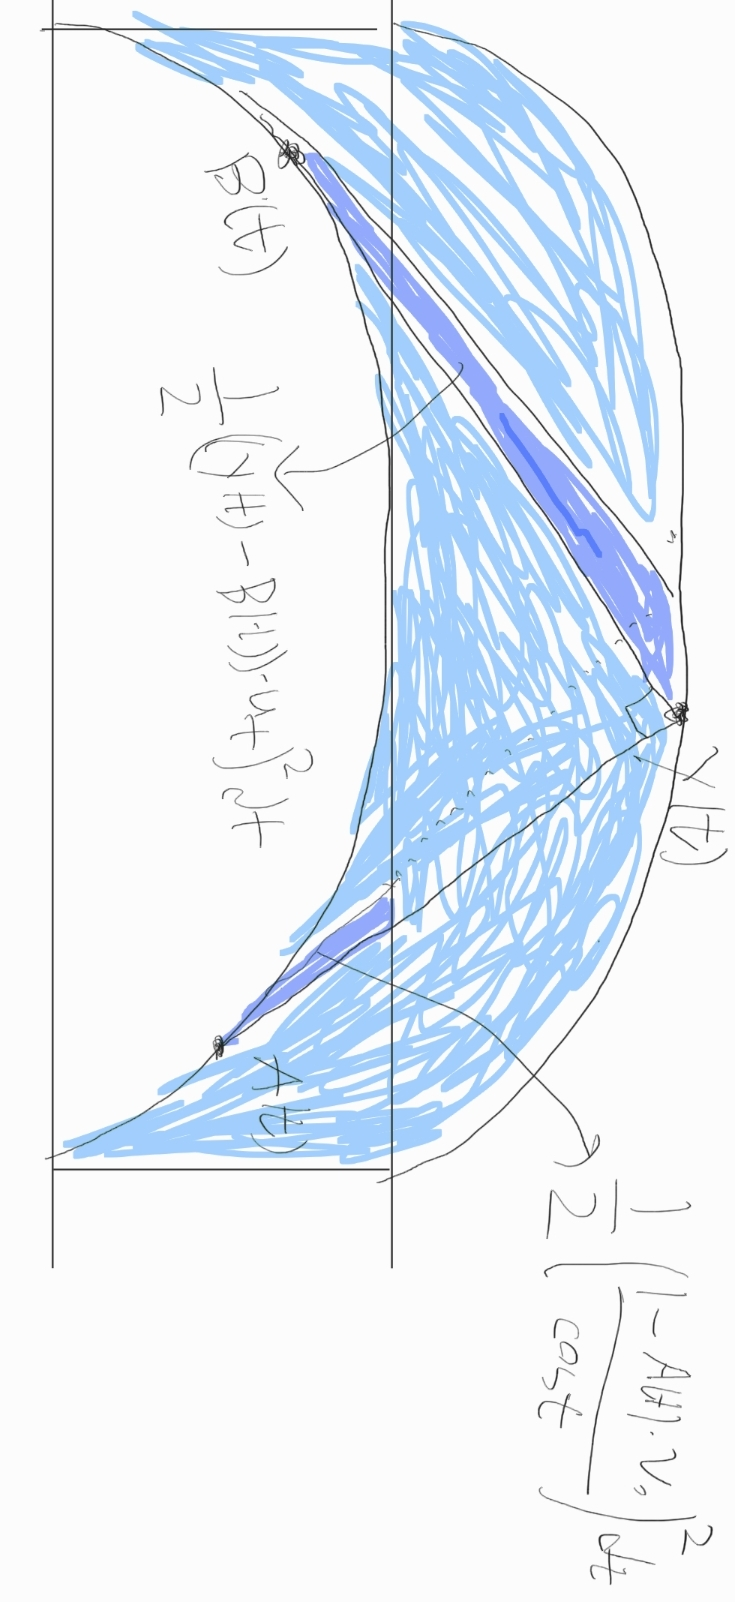
\includegraphics[width=10cm]{sofa.jpeg}
  \label{fig:test}
\end{figure}
One needs to use $h(\pi / 2) = 1$ to show this.
The integral form shows that $\cA_1$ is concave, which makes it subject to convex optimization.


\bibliographystyle{alpha}

\bibliography{references}

\end{document}
